% !TeX encoding = UTF-8
% !TeX spellcheck = de_DE
%Dokumentenklasse: Papierformat, Schriftgröße, Doppelseitig
\documentclass[12pt,a4paper,twoside]{article}

%-----------------------------------------------------------------------------------------------------------------------------
%Bestimmt die Sprache der autom. eingefügten Worte, z. B. Inhaltsverzeichnis
%Letztgenannte Sprache ist aktiv
%Wechsel mit \selectlanguage{USenglish} im Dokument möglich
\usepackage[USenglish, ngerman]{babel}
%Einstellung der Randabstände
\usepackage[left={2.5cm},right={2.5cm},top={2cm},bottom={2.5cm}]{geometry}
%Schriftart
\usepackage{helvet}
%Textverschönerungen
\usepackage{lmodern}
\usepackage{microtype}
%Einbindung von Graphiken
\usepackage{graphicx}
%Bearbeitung von Kopf- und Fusszeile
\usepackage{fancyhdr}
%Aktivierung verschiedener Umgebungen, in denen der Mathematikmodus aktiv ist
\usepackage{mathtools}
\usepackage{amsthm}
\usepackage{amsmath}
\usepackage{amssymb}
%aktiviert Hyperlinks
\usepackage[pageanchor=false]{hyperref}
%Übersetzt die Tastatureingaben für LaTex
\usepackage[utf8]{inputenc} %Bei Umlautproblemen unter MacOS: \usepackage[applemac]{inputenc}
\usepackage[T1]{fontenc}
%Stellt das Eurozeichen € (\euro) zu Verfügung
\usepackage{eurosym}
%Textbox
\usepackage{fancybox}
%Farbe
\usepackage{xcolor}
%Todo-Markierungen hinzufügen
\usepackage{todonotes}
%\usepackage[disable]{todonotes}

\usepackage{algorithm}
\usepackage{algpseudocode}

\usepackage{subfig}

%Zeilenabstand
\renewcommand{\baselinestretch}{1.24}
%Text nicht einrücken
\setlength{\parindent}{0pt}
%Fuß- und Kopfzeile
\fancyhf{}
\setlength{\headheight}{15pt}
\fancyhead[LE,RO]{\thepage}
\fancyhead[RE,LO]{\nouppercase{\rightmark}}
%Die ersten Seiten bekommen keine Kopf- oder Fußzeilen bis der "pagestyle" geändert wird
\pagestyle{empty}

%Befehle
\newtheorem{satz}{Satz}
\newtheorem{lemma}[satz]{Lemma}
\newtheorem{folgerung}[satz]{Folgerung}
\theoremstyle{definition}
\newtheorem{definition}[satz]{Definition}
\numberwithin{equation}{section}
\renewcommand{\proofname}{Beweis}
\definecolor{kitfarbe}{rgb}{0.004,0.588,0.51}
%Stellt nun auch die Eingabe "€" zur Verfügung
\DeclareUnicodeCharacter{20AC}{\euro}



\begin{document}
%-----------------------------------------------------------------------------------------------------------------------------
%Titelseite
\begin{titlepage}
  
\begin{center}
%	\includegraphics[scale=0.8]{kit_logo_de_farbe_positiv.jpg} 
	
\includegraphics[scale=0.8]{KITlogo_4c_deutsch_RGB.pdf} 

\vspace{1cm}

	\Large{
	Fakultät für Wirtschaftswissenschaften \\
	Institut für Operations Research (IOR) \\
	Diskrete Optimierung und Logistik \\
	Prof. Dr. Stefan Nickel}  
     
\vspace{1cm}

	\Large Seminararbeit % Seminararbeit, Bachelorarbeit oder Masterarbeit      
 
\vspace{1cm}
    
\setlength{\fboxrule}{3pt}

\begin{center}
\fcolorbox{kitfarbe}{white}{
	\parbox[c][3.5cm][c]{10cm}{ 
	\begin{center}
	\LARGE{Optimierung von Flugrouten unter kinematischen Nebenbedingungen} \\
	\end{center}
	}}
\end{center}

\vspace{1cm}

	von \\
	Maximilian Volk \\
	Matr. Nr.: 2101315\\
	Wirtschaftsingenieurwesen M.Sc. \\

\vspace{1cm}

	Datum der Abgabe\\
	14.01.2022

\vspace{1cm}
	
	Betreuung: \\
	M.Sc. Fabian Meyer 
    
\end{center}
  
\end{titlepage}

\cleardoublepage
%-----------------------------------------------------------------------------------------------------------------------------
%Eidesstattliche Erklärung
\vspace*{1cm}

{\Large \textbf{Eidesstattliche Erklärung}} 

\bigskip

Ich versichere hiermit wahrheitsgemäß, die Arbeit selbständig angefertigt, alle benutzten Hilfsmittel vollständig und genau angegeben und alles kenntlich gemacht zu haben, was aus Arbeiten anderer unverändert oder mit Abänderung entnommen wurde.\\
\vspace{1cm}

\textit{Datum} \hspace{8cm} \textit{Name}

\cleardoublepage
%-----------------------------------------------------------------------------------------------------------------------------
%Seitennummerierungen und Inhaltsverzeichnis
\rmfamily \pagestyle{fancy}
\renewcommand{\sectionmark}[1]{\markright{\thesection\ #1}}
\setcounter{secnumdepth}{4}
\pagenumbering{roman} \setcounter{page}{3} 
\tableofcontents
\newcounter{roemisch} \setcounter{roemisch}{\value{page}}
\clearpage
\mbox{}\thispagestyle{empty}\clearpage
\setcounter{page}{2} \pagenumbering{arabic}
%-----------------------------------------------------------------------------------------------------------------------------
%Beginn der Arbeit
\section{Einleitung}\label{section:introduction}
Ein wichtiges Einsatzgebiet unbemannter Luftfahrzeuge (engl. unmanned aereal vehicles, UAVs) sind zivile oder militärische Aufklärungsflüge. Sollen mehrere Ziele mit einem unbemannten Luftfahrzeug abgeflogen werden, stellt sich die Frage nach der optimalen Abflugreihenfolge der Ziele. Das Problem eine gegebene Menge an Zielen in möglichst geringer Zeit oder zu minimalen Kosten aufzusuchen ist als Problem des Handlungsreisenden (engl. Traveling Salesman Problem, TSP) bekannt und eines der meistuntersuchten kombinatorischen Optimierungsprobleme. In Anwendungen ist allerdings häufig die Rolle von Zielfunktion und Nebenbedingung gegenüber dem TSP vertauscht. Erstens müssen häufig nicht zwingend alle Ziele besucht werden, sondern das Auslassen eines Ziels geht mit bestimmten Kosten einher oder äquivalent geht das Besuchen eines Ziels mit einer Belohnung einher. Zweitens reicht das vorhandene Zeitbudget nicht für das Besuchen aller Ziele aus, sodass zwangsläufig eine Auswahl getroffen werden muss, welche Ziele zu besuchen sind.\\

Diese Problemstellung, bei der innerhalb eines bestimmten Zeitrahmens möglichst gewinnbringend Ziele aus einer Menge zu besuchen sind, wurde erstmals 1984 von Tsiligirides \cite{Tsiligirides.1984} untersucht. Das Problem wird nach der Sportart des Orientierungslaufs (engl. Orienteering) meist als Orienteering Problem (OP) bezeichnet, allgemeiner wird auch der Begriff des Routing Problem with Profits \cite{Vansteenwegen.2019} verwendet.
Neben der Bestimmung einer optimalen Tour, in der alle Ziele einer bestimmten Teilmenge besucht werden müssen, die der Lösung eines TSP entspricht, ist im OP zusätzlich die Auswahl der entsprechenden Teilmenge an Zielen nötig, was dem Rucksackproblem entspricht. Sowohl das TSP als auch das Rucksackproblem sind NP-schwere Probleme, sodass das Orienteering Problem, welches beide als Subprobleme enthält, ebenfalls mindestens ein NP-schweres Problem ist.\\

Sowohl beim TSP als auch beim klassischen OP sind paarweise Distanzen für alle Ziele bekannt und es werden keine weiteren Restriktionen an den optimalen Pfad gestellt. Ein Luftfahrzeug ist allerdings nicht beliebig manövrierbar und kann daher nicht jeden Pfad, der eine Lösung darstellt, tatsächlich abfliegen. Vielmehr genügt jeder tatsächlich abfliegbare Pfad eines Luftfahrzeug bestimmten kinematischen Restriktionen. Um diese Restriktionen angemessen zu berücksichtigen, wird ein kinematisches Modell des Luftfahrzeugs benötigt. 

In dieser Arbeit wird das Luftfahrzeug als Dubinsfahrzeug (engl. Dubins vehicle) \cite{Dubins.1957} modelliert. Dabei handelt es sich um ein Fahrzeug, welches nur solche Pfade abfliegen kann, deren Krümmung kleiner als eine bestimmte maximal zulässige Krümmung ist. Die Pfade minimaler Distanz eines solchen Fahrzeugs zwischen zwei Zielen werden als Dubinspfade bezeichnet. Aufgrund der Krümmungsrestriktion ergibt sich je nach Ausrichtungen des Fahrzeugs an den Zielen ein unterschiedlicher Dubinspfad. Die Distanz zwischen zwei Zielen ist also abhängig von der Start- und Endausrichtung des Fahrzeugs welche wiederum die angrenzenden Dubinspfade und Distanzen beeinflussen. Mit dieser Distanzdefinition in der Ebene wird das Orienteering Problem zum Dubins Orienteering Problem (DOP). Die im DOP zusätzlich optimal zu bestimmenden  Ausrichtungen des Fahrzeugs an jedem besuchten Ziel erhöhen die Komplexität des Problems zusätzlich.

% Versuchte man mit einem Dubinsfahrzeug den Pfad einer Lösung des EOP abzufliegen, verfügt dieser über Ecken

Erstmals untersucht wurde das DOP 2017 von Penicka et al. (\cite{R.Penicka.2017}), welche auch ein heuristisches Lösungsverfahren angeben, das eine Adaption der variablen Nachbarschaftssuche darstellt.\\

Ziel dieser Arbeit ist es, das Dubins Orienteering Problem und das darauf angepasste Verfahren der variablen Nachbarschaftssuche vorzustellen. Anhand einer eigenen Implementierung des Verfahrens sowie dessen Anwendung auf Beispielinstanzen werden dessen Eigenschaften analysiert. Zuletzt werden eigene Verbesserungen für das Verfahren vorgeschlagen.


\newpage
\section{Literatur}\label{section:literature}
Bei der ersten Vorstellung des Orienteering Problems in \cite{Tsiligirides.1984} gibt Tsiligirides auch zwei Konstruktionsheuristiken - eine stochastische und eine deterministische - sowie eine Verbesserungsheuristik an. Daneben gibt er drei Probleminstanzen an, welche auch in dieser Arbeit zur Evaluation numerischer Verfahren herangezogen werden.

Tsiligirides selbst bezeichnet die Problemstellung als Generalized Travelling Salesman Problem. Der in der Literatur heute standardmäßig verwendete Begriff des Orienteering Problems wird erstmals 1987 von Golden et al. \cite{Golden.1987} eingeführt, welche als Lösungsverfahren eine Heuristik entwickeln, die auf aus den Koordinaten der Ziele berechneten Schwerpunkten basiert.

Chao et al. \cite{Chao.1996b} stellen ein weiteres Verfahren vor, welches zur Verbesserung einer gefundenen Lösung neben dem Verschieben und Austauschen zweier Ziele in der Lösung die 2-Opt-Operation einsetzt. Daneben werden Probleminstanzen angegeben, von denen zwei, genannt Set 64 und Set 66, in der Arbeit von Penicka et al. \cite{R.Penicka.2017} betrachtet werden.

Neben diesem klassischen Orienteering Problem existieren weitere Varianten, von denen einige wichtige hier kurz genannt werden sollen. Chao et al. \cite{Chao.1996} stellen 1996 das Team Orienteering Problem (TOP) vor, bei dem mehrere Teammitglieder gemeinsam möglichst viele Belohnungen einsammeln. Sind zusätzlich noch Zeitfenster für die Besuche bestimmter Ziele zu berücksichtigen, spricht man vom (Team) Orienteering Problem with Time Windows ((T)OPTW) \cite{Vansteenwegen.2019}.

Noch allgemeiner werden all jene Probleme, bei denen nicht alle Ziele aus einer Menge besucht werden müssen, als Routing Problems with Profits bezeichnet. Dazu zählen neben der Familie der Orienteering Probleme auch das Profitable Tour Problem (PTP), bei dem im Gegensatz zum OP die Bewegung zwischen Zielen Kosten verursacht, welche in die Zielfunktion eingehen und das Prize-Collecting Traveling Salesman Problem (PCTSP). Weiterhin gibt es Routing Probleme mit mehreren Zielfunktionen, Kapazitätsbeschränkungen und zeitabhängigen Belohnungen. Eine Übersicht über diese Routing Probleme wird in \cite{Vansteenwegen.2019} gegeben.

Das in dieser Arbeit untersuchte und 2017 von Penicka et al. \cite{R.Penicka.2017} vorgestellte Dubins Orienteering Problem ist das erste OP, in dem kinematische Nebenbedingungen berücksichtigt werden. Die kinematischen Nebenbedingungen ergeben sich dabei aus der Modellierung des Fahrzeugs als Dubinsfahrzeug. In diesem kinematischen Modell bewegt sich das Fahrzeug mit konstanter Geschwindigkeit und mit einem minimalen Kurvenradius. 

1957 zeigte Dubins \cite{Dubins.1957}, dass in diesem Modell die kürzesten Pfade zwischen zwei Punkten in der Ebene nur aus drei Segmenten bestehen. Da diese relativ leicht zu bestimmen sind, existieren zur Planung dieser Pfade mehrere Implementierungen, beispielsweise in Python \cite{AtsushiSakai.2018}. 

Penicka et al. stellen in einer weiteren Arbeit \cite{R.Penicka.2017b} das Dubins Orienteering Problem with Neighbourhoods (DOPN) vor, bei dem es für den Erhalt der Belohnung eines Ziels ausreichend ist, an diesem innerhalb eines gewissen Abstandes vorbeizufliegen. Erstmals in einem Routing Problem angewendet wurde das kinematische Modell von Dubins allerdings bereits 2005 von Savla et al. \cite{K.Savla.2005} als Dubins Traveling Salesperson Problem (DTSP).

Neben den eingangs erwähnten Verfahren von Tsiligirides \cite{Tsiligirides.1984}, Golden et al. \cite{Golden.1987} und Chao et al. \cite{Chao.1996b} stellten Ramesh et al. \cite{Ramesh.1991} eine vierphasige Heuristik vor. Bei dieser werden phasenweise Ziele aus der Lösung hinzugefügt und entfernt, je nach dem jeweiligen Verhältnis zwischen der zusätzlichen Belohnung und der zusätzlicher Distanz welche ein einzelnes Ziel zur Lösung beiträgt.

Die weiteren zur Lösung des OP eingesetzten heuristischen Verfahren lassen sich in solche, die eine Population von Lösungen und solche, welche eine einzelne Lösung parallel verwenden, unterteilen. Zu Ersteren zählen beispielsweise eine diskrete Variante der Partikelschwarmoptimierung \cite{Z.Sevkli.2010} sowie evolutionäre Algorithmen \cite{Kobeaga.2018}. Zur Lösung des OP eingesetzte Verfahren, die eine einzelne Lösung iterativ verbessern sind beispielsweise die Tabu Search \cite{Gendreau.1998}, die Adaptive Large Neighbourhood Search (ANLS) \cite{Santini.2019} sowie die Variable Neighbourhood Search \cite{Sevkli.2006}. Weitere Verfahren zur Lösung des OP finden sich in den Übersichtsarbeiten \cite{Vansteenwegen.2011} und \cite{Gunawan.2016}.

Die von Hansen und Mladenovic \cite{Hansen.2001} allgemein sowie insbesondere für das TSP diskutierte und von Sevkli et al. \cite{Sevkli.2006} auf das OP angewendete Variable Neighbourhood Search wird in der dieser Arbeit zugrundeliegenden Arbeit von Penicka et al. \cite{R.Penicka.2017} zur Lösung des DOP weiterentwickelt. Penicka et al. \cite{R.Penicka.2017} vergleichen sie für reguläre OPs mit der Heuristik von Chao et al. \cite{Chao.1996b}, der vierphasigen Heuristik \cite{Ramesh.1991} sowie der ursprünglichen Variable Neighbourhood Search \cite{Sevkli.2006}, wobei als Testinstanzen Set 1, 2 und 3 von Tsiligirides \cite{Tsiligirides.1984} sowie Set 64 und 66 von Chao et al. \cite{Chao.1996b} dienen.

\newpage

\section{Problemstellung}\label{section:problem}
In diesem Abschnitt soll zunächst das Orienteering Problem formal beschrieben werden. Anschließend wird das kinematische Modell des Dubinsfahrzeugs vorgestellt und zuletzt das sich daraus ergebende Dubins Orienteering Problem diskutiert.
Der folgende Abschnitt orientiert sich an \cite{Vansteenwegen.2019} und verwendet die Notation aus \cite{R.Penicka.2017}.

\subsection{Orienteering Problem}\label{subsection:OP}

Wie in der Einleitung beschrieben, bezeichnet das Orienteering Problem die Aufgabe aus einer Menge von Zielen $I = \{1,...,n\}$  mit Belohnungen $r_i \geq 0$, die beim Besuchen eines Ziels $i \in I$ erhalten werden, eine Teilmenge dieser Zielen zu besuchen, sodass die Summe der Belohnungen dieser Ziele maximal wird und der dafür notwendige Pfad, beginnend bei $i = 1$ und endend bei $ i = n$, nicht länger als das Streckenbudget $T_{max}$ ist.
Es handelt sich beim Orienteering Problem um ein NP-schweres Problem \cite{Vansteenwegen.2019}.

Die paarweisen Distanzen $t_{ij}, i,j\in I$ sowie das Budget $T_{max}$ werden meist in Zeiteinheiten ausgedrückt, Längeneinheiten sind aber ebenso möglich. Generell wird angenommen, dass die Belohnungen von Start- und Endziel null sind $r_1 = r_n = 0$ und die aller anderen Ziele strikt positiv, also $r_i > 0, 1 < i < n$. In diesem Fall können übereinstimmende Start- und Endziele über eine entsprechende Definition der Distanzen zu diesen Zielen in der Formulierung berücksichtigt werden.

Unter Verwendung der Notation $\mathcal{S}(I)$ für die Menge aller Permutationen der Menge $I$ lässt sich eine zulässige Lösung des Orienteering Problem als Permutation $\Sigma = (\sigma_1,...,\sigma_n) \in \mathcal{S}(I)$ beschreiben, versehen mit $k \in I$, sodass
\begin{equation}
	\sum_{i = 2}^{k} t_{\sigma_{i-1}\sigma_{i}} \leq T_{max}
\end{equation}
sowie $\sigma_1 = 1$ und $\sigma_k = n$ gilt. Den gesuchten Pfad bilden dann die Ziele $\sigma_1,...,\sigma_k$. Obwohl sie nicht Teil des eigentlich gesuchten Pfades sind, stellen die Ziele, welche in der Permutation hinter $\sigma_k$ stehen, einen Teil der Lösung dar. Insbesondere die Information über ihre Position wird in Lösungsverfahren verwendet, wie später gezeigt wird.

Mit diesen Definitionen lässt sich das Orienteering Problem schreiben als
\begin{align}
	\begin{array}{llcll}
		\text{max}  & \sum_{i=1}^{k} r_{i}        &      &             & \\
		\text{s.t.} & \sum_{i = 2}^{k} t_{\sigma_{i-1}\sigma_{i}}    & \leq    &  T_{max}         &  \\
		& \sigma_1 & = & 1 & \\
		& \sigma_k & = & n     &\\
		& \Sigma & \in & \mathcal{S}(I) & \\
		& k & \in & I & 
	\end{array}
	\tag{OP}
	\label{OP}
\end{align}

In \cite{R.Penicka.2017} sind die Ziele $i \in I$ mittels ihrer Position in der Ebene $s_i \in \mathbb{R}^2$ identifiziert. Statt des zeitlichen Abstandes wird die euklidische Distanz zwischen zwei Zielen $i,j$, bezeichnet mit $\mathcal{L}_{e}(s_i,s_j)$, verwendet. Entsprechend ist $T_{max}$ kein Zeit- sondern ein Streckenbudget. Das Orienteering Problem mit dieser Distanzdefinition wird als Euklidisches Orienteering Problem (EOP) bezeichnet. Eine zulässige Lösung ($\Sigma,k$) des EOP erfüllt folglich
\begin{equation}
	\sum_{i = 2}^k \mathcal{L}_{e}(s_{\sigma_i},s_{\sigma_j}) \leq T_{max}
\end{equation}

Mit dieser Schreibweise können neben der euklidischen Metrik noch andere Distanzmaße verwendet werden. Beispiele hierfür sind die Manhattan- oder Maximumsmetrik. Bei dem in dieser Arbeit untersuchten Dubins Orienteering Problem wird als Distanzmaß die Länge des kürzesten Wegs eines Dubinsfahrzeugs verwendet.
Eine Formulierung des Orienteering Problem als ganzzahliges lineares Programm ist in \cite{Vansteenwegen.2019} zu finden.

\subsection{Dubinsfahrzeug}\label{subsection:Dubinsvehicle}
In dieser Arbeit dient das Dubinsfahrzeug als Modell des unbemannten Luftfahrzeugs. Ein Dubinsfahrzeug wird dadurch charakterisiert, dass es sich mit konstanter Geschwindigkeit $v$ vorwärts bewegt und einen minimalen Kurvenradius $\rho$ hat, wodurch Pfade dieses Fahrzeugs höchstens eine Krümmung von $\frac{1}{\rho}$ aufweisen.
Der Zustand eines Dubinsfahrzeug zu einem beliebigen Zeitpunkt ist $q = (x,y,\theta)$ wobei $(x,y) \in \mathbb{R}^2$ die Position in der Ebene und $\theta \in [0,2\pi]$ die Ausrichtung des Fahrzeugs angibt. Das kinematische Modell des Dubinsfahrzeug lässt sich folgendermaßen ausdrücken
\begin{equation}
	\dot{q} = \begin{bmatrix} \dot{x}\\
		\dot{y}\\
		\dot{\theta}
	 \end{bmatrix} 
 = \begin{bmatrix} \cos(\theta)\\
	 \sin(\theta)\\
	 \frac{u}{\rho}
 \end{bmatrix}, u \in [-1,1] 
\label{DubinsModel}
\end{equation}
wobei mit $u$ die aktuelle Ausrichtung gesteuert wird und $\dot{f} := \frac{df}{dt}$ die Ableitung einer Funktion $f(t)$ nach der Zeit $t$ bezeichnet.

Dubins \cite{Dubins.1957} zeigte, dass sich der kürzeste Pfad und dessen Länge $\mathcal{L}_d(q_1,q_2)$ zwischen zwei Zuständen $q_1,q_2$ im Modell~(\ref{DubinsModel}) stets eines der sechs Manöver $\{LSL,LSR,RSL,RSR,LRL,RLR\}$, genannt Dubinsmanöver, ist, wobei $S$ eine gerade Strecke und $L$ bzw. $R$ Kurven mit Radius $\rho$ bezeichnen. Ein Dubinsfahrzeug bewegt auf einem kürzesten Pfad also stets entweder auf einer Geraden ($u = 0$) oder auf einer Kurve mit maximaler Krümmung ($u \in \{1,-1\}$). Zwei beispielhafte Dubinspfade sind in Abbildung~\ref{fig:DubinsPaths.png} dargestellt, die \cite{LaValle.2006} entnommen ist. Dort finden sich noch weitere Erklärungen der Dubinsmanöver und zugehörige Literatur.

\begin{figure}[h]
	\begin{center}
		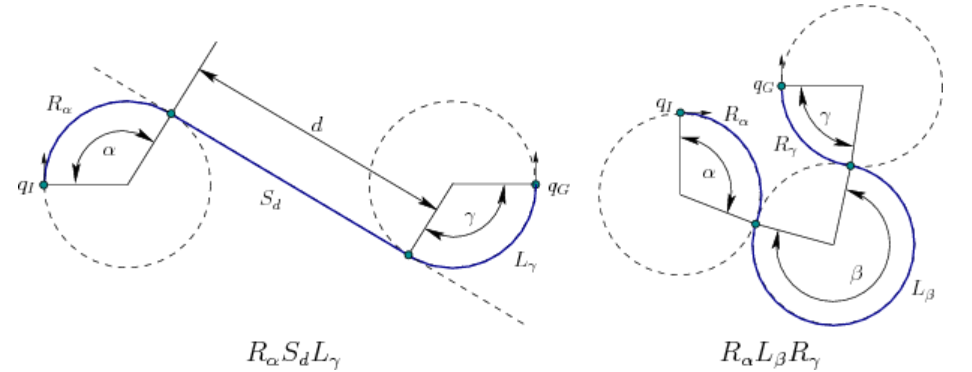
\includegraphics[scale=0.8]{DubinsPaths.png}
	\end{center}
	\caption{Zwei beispielhafte Dubinsmanöver}
	\label{fig:DubinsPaths.png}
\end{figure}


\subsection{Dubins Orienteering Problem}\label{subsection:DOP}
Indem im EOP die euklidische Distanz zwischen zwei Zielen durch die Länge $\mathcal{L}_d$ des Dubinspfads ersetzt wird, entsteht das Dubins Orienteering Problem (DOP). Allerdings ist die Dubinsdistanz $\mathcal{L}_d$ nicht nur von der Position $s_i$ des Ziels $i \in I$ sondern auch von der dortigen Ausrichtung $\theta_i$ des Dubinsfahrzeugs abhängig. Somit setzt sich eine Lösung des DOP neben der Permutation $\Sigma$ und dem Index $k\in I$ des Endziels $n$ in $\Sigma$ auch aus den Ausrichtungen $\Theta = (\theta_{\sigma_1},...,\theta_{\sigma_k})$ an den ersten $k$ Zielen zusammen.

Im Folgenden wird eine Lösung des DOP mit $P = (\Sigma,k,\Theta)$ bezeichnet. Für die Länge und Gesamtbelohnung einer Lösung wird kurz $\mathcal{L}_d(P) = \sum_{i = 2}^k \mathcal{L}_{d}(q_{\sigma_i},q_{\sigma_j})$ bzw. $R(P) = \sum_{i = 1}^k r_i$ geschrieben. Hierbei ist $q_i = (s_{i},\theta_{i})$ der Zustand des Dubinsfahrzeugs am Ziel $i\in I$.
Eine zulässige Lösung erfüllt entsprechend $\mathcal{L}_d(P)\leq T_{max}$.

Insgesamt hat das DOP die folgende Form:

\begin{align}
	\begin{array}{llcll}
		\text{max}  & \sum_{i=1}^{k} r_{i}        &      &             & \\
		\text{s.t.} & \sum_{i = 2}^{k} \mathcal{L}_d(q_{\sigma_{i-1}},q_{\sigma_{i}})   & \leq    &  T_{max}         &  \\
		& \sigma_1 & = & 1 & \\
		& \sigma_k & = & n     &\\
		& \Sigma & \in & \mathcal{S}(I) & \\
		& k & \in & I & 
	\end{array}
	\tag{DOP}
	\label{DOP}
\end{align}

Da im Vergleich zum OP im DOP noch zusätzlich die optimalen Ausrichtungen $\Theta$ bestimmt werden müssen, ist dass DOP noch schwerer zu lösen und insbesondere ebenfalls NP-schwer.

\begin{figure}[ht]
	\centering
	\subfloat[\centering Zulässige Lösung für $\rho = 0$, $T_{max} = 70$ mit Belohnung $R(P) = 600$ und Distanz $\mathcal{L}_d(P) = 69.4406$ ]{{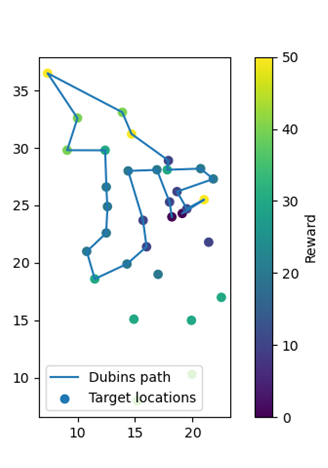
\includegraphics[height=6.3cm]{Set3_Dubinspath_rad0_T70.png} }}%
	\qquad
	\subfloat[\centering Zulässige Lösung für $\rho = 1$, $T_{max} = 70$ mit Belohnung $R(P) = 570$ und Distanz $\mathcal{L}_d(P) = 68.6386$ ]{{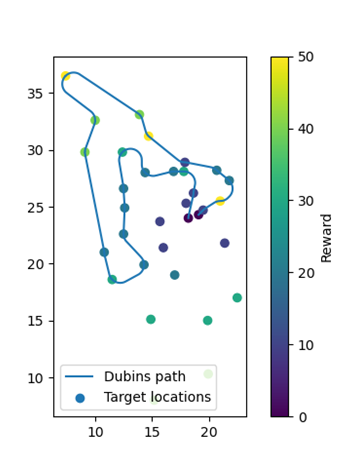
\includegraphics[height=6.3cm]{Set3_Dubinspath_rad1_T70.png} }}%
	\qquad
	\subfloat[\centering Zulässige Lösung für $\rho = 3$, $T_{max} = 70$ mit Belohnung $R(P) = 320$ und Distanz $\mathcal{L}_d(P) = 66.5065$
	]{{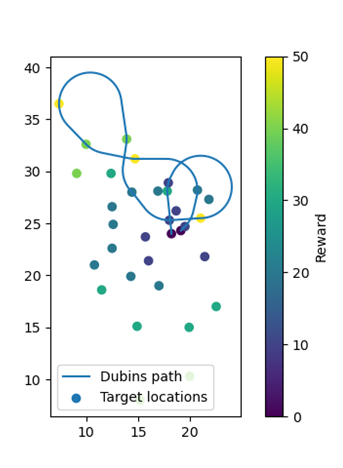
\includegraphics[height=6.3cm]{Set3_Dubinspath_rad3_T70.png} }}%
	\caption{Probleminstanz Set 3 des OP/DOP mit zulässigen Lösungen}
	\label{fig:Set3_Dubinspath_rad013.png}
\end{figure}

Die von Tsigilirides \cite{Tsiligirides.1984} vorgestellte OP Beispielinstanz Set 3 ist in Abbildung~\ref{fig:Set3_Dubinspath_rad013.png} dargestellt. Dabei sind für die minimalen Radien des Dubinsfahrzeugs $\rho \in \{0,1,3\}$ jeweils eine zulässige Lösung des DOP dargestellt. Für $\rho = 0$ enstpricht das DOP gerade dem EOP bzw. OP entspricht.

\clearpage

\section{Lösungsverfahren}\label{section:Loesungsverfahren}
Bereits zum Lösen des OP kommen in praktischen Anwendungen meist heuristische Verfahren zum Einsatz \cite{Vansteenwegen.2011}, wenn auch mit Branch-and-Cut-Verfahren bereits Instanzen mit bis zu 500 Zielen exakt gelöst werden konnten \cite{Fischetti.1998}. Daher liegt es nahe, zu Lösung des noch schwereren DOP ebenfalls heuristische Verfahren einzusetzen, um in akzeptabler Zeit gute Lösungen zu erhalten.

Das von Penicka et al. in \cite{R.Penicka.2017} zur Lösung des DOP verwendete Verfahren ist eine Adaption des Verfahrens der variablen Nachbarschaftssuche (Variable Neighbourhood Search (VNS)). Dieses von Hansen und Mladenovic \cite{Hansen.2001} entwickelte Verfahren stellt eine Metaheuristik für kombinatorische Optimierungsprobleme dar. Die Grundidee des Ansatzes ist es, die in einem lokalen Suchverfahren eingesetzte Nachbarschaft hinsichtlich ihrer Struktur und Größe im Laufe des Verfahrens systematisch zu verändern. Damit soll verhindert werden sich in einem lokalen Optimum, welches nicht global optimal ist, zu verfangen.

\subsection{Konstruktion einer zulässigen Lösung}\label{subsection:construction}
Bevor die eigentliche Verbesserung einer Lösung im Rahmen der VNS erfolgen kann, muss zunächst eine initiale zulässige Lösung konstruiert werden. Im Folgenden soll das Verfahren, welches Penicka et al. \cite{R.Penicka.2017} hierfür vorschlagen, erläutert werden. 

Dafür werden in \cite{R.Penicka.2017} zunächst diejenigen Ziele ausgeschlossen, die für sich genommen bereits mit dem gegebenen Streckenbudget $T_{max}$ nicht erreichbar sind. Diese Idee stammt von Chao et al. \cite{Chao.1996b}, welche diese Vorauswahl in ihrer Heuristik für das OP einführen. Aufgrund der euklidischen Distanzen liegen im OP alle so ausgewählten Ziele innerhalb einer Ellipse, deren Brennpunkte das Start- und Endziel sind und deren Hauptachse die Länge $T_{max}$ hat. Da die Distanzen der Dubinspfade von den Ausrichtungen $\Theta$ abhängen, muss bei der Anwendung dieser Einschränkung entschieden werden, ob neben denjenigen Zielen, welche für alle Ausrichtungskombinationen von Start, Ziel und Endziel nicht erreichbar sind, bereits all jene auszuschließend sind, für die eine Ausrichtungskombination existiert, sodass das Budget überschritten wird. Penicka et al. \cite{R.Penicka.2017}  schließen hier alle Ziele, welche nicht für alle Ausrichtungswinkel zulässig sind, aus, ungeachtet dessen, dass so möglicherweise hilfreiche Ziele ausgeschlossen werden. Die Bedingung, welche die Menge $I_r$ der erreichbaren Ziele charakterisiert lautet also
\begin{equation*}\label{eq:I_r}
	i \in I_r \Leftrightarrow \mathcal{L}_d(q_{1},q_{i}) + \mathcal{L}_d(q_{i},q_{n}) \leq    T_{max} \ \forall (\theta_1,\theta_i,\theta_{n}) \in (\Theta^m)^3.
\end{equation*}
Um nur diejenigen Ziele auszuschließen, für die keine zulässige Kombination von Ausrichtungen existiert, wird der Allquantor in (\ref{eq:I_r}) durch den Existenzquantor ersetzt.

Gerade für größere Kurvenradien $\rho$ und kleine Budgets $T_{max}$ lassen sich Ausrichtungswinkel finden, die in eine ungünstige Richtung zeigen, sodass ein Ziel für sich genommen ausgeschlossen wird, obwohl es sogar zur optimalen Lösung gehört. Im folgenden wird daher auch untersucht, inwiefern sich der Zielfunktionswert der initial konstruierten Lösung abhängig von diesem Ausschluss verändert.

Aus den übrigen Zielen wird, ausgehend von einem zunächst direkten Pfad von Ziel 1 nach $n$, jeweils dasjenige Ziel hinzugefügt, welches die größte zusätzliche Belohnung je zusätzlicher Strecke beiträgt. Dabei werden für jedes solche Ziel bereits die optimale Einfügeposition und alle optimalen Ausrichtungswinkel bestimmt und berücksichtigt. Es werden Ziele auf diese Weise zum Pfad hinzugefügt, solange das Streckenbudget $T_{max}$  nicht überschritten wird.\\

\subsection{Verbesserung der Lösung}\label{subsection:improvement}
Für die Variation der Nachbarschaft im Rahmen der VNS müssen zunächst problemspezifisch endlich viele Nachbarschaftsstrukturen $N_l, l = 1,...,l_{max}$ definiert werden, wobei $N_l(P)$ für eine Lösung $P$ die Menge aller Lösungen in der Nachbarschaft $N_l$ um $P$ bezeichnet.

Auf eine initial konstruierte zulässige Lösung $P$ werden iterativ für alle Nachbarschaftsstrukturen $N_l$, beginnend bei $l = 1$ aufsteigend bis $l_{max}$ die zwei Operatoren \textit{shaking} und \textit{local search} angewendet.

Beim $\textit{shaking}$ wird innerhalb der Nachbarschaft $N_l(P)$ zufällig eine zulässige Lösung $P'$ ausgewählt. Dieser Schritt dient dem Ausbrechen aus einem lokalen Optimum. Anschließend wird eine lokale Suche (\textit{local search}) mit $P'$ als initialer Lösung durchgeführt, deren Ergebnis $P''$ ist.
Bei dieser lokalen Suche weichen Penicka et al. \cite{R.Penicka.2017} allerdings von der klassischen VNS ab. Statt einer gewöhnlichen lokalen Suche, bei der systematisch die beste Lösung in der aktuellen Nachbarschaft ausgewählt wird, setzen sie auf ein randomisiertes Verfahren. Lediglich eine bestimmte Anzahl an Iterationen lang wird versucht die Lösung innerhalb der aktuellen Nachbarschaft zu verbessern. Die Autoren der zugrundeliegenden Arbeit schlagen als Iterationszahl für die lokale Suche $|I|^2$ vor.

Das resultierende Verfahren wird auch als Randomized Variable Neighbourhood Search (RVNS) bezeichnet. Begründet wird die Verwendung der RVNS für das DOP mit der größeren Schnelligkeit gegenüber der regulären VNS bei gleichen erzielten Belohnungen im Falle des OP \cite{Sevkli.2006}.

Wenn das gefundene lokale Optimum $P''$ zulässig ist und über eine höhere Belohnung verfügt als die bisherige Lösung $P$, wird diese durch $P''$ ersetzt und ausgehend von der neuen besten Lösung das Verfahren in der kleinsten Nachbarschaftsstruktur (d.h.$l = 1$) fortgesetzt. Andernfalls wird das Verfahren ausgehend von der bisherigen Lösung in der nächstgrößeren Nachbarschaftsstruktur ($l = l+1$) fortgeführt.

Sevkli et al. \cite{Sevkli.2006} wenden die VNS erstmals auf das Orienteering Problem an. Sie definieren die folgenden vier Nachbarschaftsstrukturen, die ihrer Größe nach aufsteigend sortiert sind:

\begin{itemize}
	\item Einfügen (Insert): Einfügen eines zufällig ausgewählten Ziels vor einem anderen zufällig ausgewählten Ziel.
	\item Austausch (Exchange): Tausch der Position zweier verschiedener zufällig ausgewählter Ziele
	\item Pfadeinfügen (Path insert): Einfügen eines zufällig ausgewählten Subpfads vor einem anderen, zufällig ausgewählten Ziel
	\item Pfadaustausch (Path exchange): Tausch der Position zweier überschneidungsfreier, zufällig ausgewählter Pfade
\end{itemize}

Wichtig zu beachten ist bei den Nachbarschaftsstrukturen, dass bei den zugrundeliegenden Operationen wie dem Einfügen und Verschieben von Zielen und Teilpfaden die gesamte Permutation $\Sigma$ betrachtet wird und nicht nur innerhalb des eigentlichen Pfads Ziele bewegt werden. In diesem Fall könnte sich nur die Reihenfolge der ausgewählten Ziele verändern. Wird hingegen die ganze Permutation herangezogen, kann sich neben Reihenfolge der ausgewählten Ziele auch deren Zusammensetzung ändern. Es können nichtausgewählte Ziele, die sich hinter $\sigma_k = n$ in der Permutation befinden hinzugefügt werden, sowie ausgewählte Ziele aus dem eigentlichen Pfad entfernt werden, indem diese in jenen hinteren Teil der Permutation wandern. Dabei ist darauf zu achten, dass Ziel 1 stets an erster Stelle in der Permutation steht und sich dessen Position durch die Operationen nicht verändert. Der eigentliche Pfad ergibt sich also aus allen Zielen, die zwischen der ersten Stelle $\sigma_1 = 1$ und der Stelle $\sigma_k = n$, an der sich das Endziel befindet, in der Permutation stehen.

Diese vier Nachbarschaftsstrukturen sind es auch, die Penicka et al. \cite{R.Penicka.2017} in ihrer variablen Nachbarschaftssuche einsetzen und auf das Dubins Orienteering Problem angewendet werden.
Beim \textit{shaking} werden die Nachbarschaftsstrukturen Pfadeinfügen, welche $l = 1$ entspricht, und Pfadaustausch, welcher $l = 2$ entspricht, verwendet. In der \textit{local search} werden für $l = 1$ das Einfügen und für $l = 2$ der Austausch eingesetzt.

Hier zeigen sich die unterschiedlichen Ziele der beiden Operatoren \textit{shaking} und \textit{local search}. Bei der lokalen Suche soll möglichst ein lokales Optimum gefunden werden, weshalb hier die beiden kleineren Nachbarschaftsstrukturen zum Einsatz kommen. Im Gegensatz dazu zielen die beiden größeren Nachbarschaftsstrukturen beim \textit{shaking}-Operator darauf ab, aus einem solchen lokalen Optimum auszubrechen. In beiden Operatoren nimmt die Größe der verwendeten Nachbarschaft im Laufe des Verfahrens zu.

Neben der Auswahl und Reihenfolge der Ziele sind beim DOP noch die Ausrichtungswinkel $\Theta$ zu bestimmen. Penicka et al. verwenden hierfür $m$ gleichverteilte Winkel aus $[0,2\pi]$ aus denen jeder der Ausrichtungswinkel ausgewählt wird. Die Menge der diskreten Winkel wird im Folgenden mit $\Theta^m$ bezeichnet. Für gegebene $\Sigma, k$ werden  diejenigen Winkel $\Theta$ ausgewählt, welche die Länge des Pfads minimieren.

Da an jedem der Ziele ein Ausrichtungswinkel ausgewählt werden muss, kann die Bestimmung der optimalen Winkel als Suche nach einem kürzesten Pfad in einem mehrstufigen Graphen aufgefasst werden. Zu jedem Ziel im Pfad der Lösung existiert eine Stufe im Graph. In jeder dieser Stufen stehen die $m$ möglichen Winkel zur Auswahl, wobei nur Knoten unmittelbar aufeinanderfolgender Stufen miteinander über eine Kante verbunden sind. Das Gewicht einer solchen Kante entspricht gerade der Länge des Dubinspfades von ihrem Start- zum Endknoten. Ein solcher Graph ist in Abbildung~\ref{fig:search_graph.png}, welche  \cite{R.Penicka.2017} entnommen ist, dargestellt.

\begin{figure}[h]
	\begin{center}
		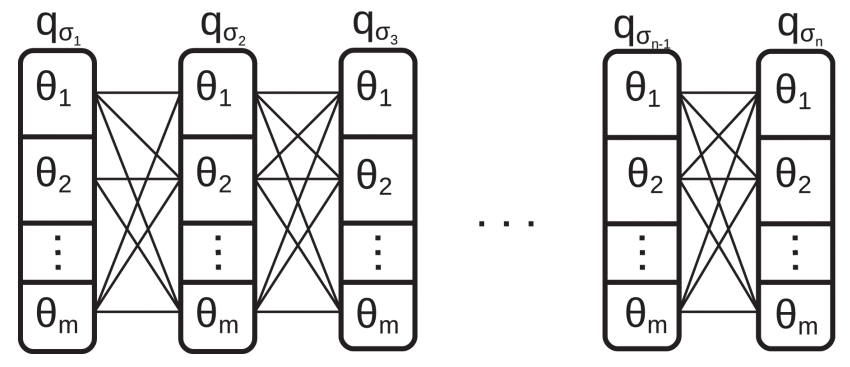
\includegraphics[scale=0.8]{search_graph.png}
	\end{center}
	\caption{Suchgraph für die Bestimmung optimaler Ausrichtungswinkel}
	\label{fig:search_graph.png}
\end{figure}

Das Verfahren der variablen Nachbarschaftssuche ist noch einmal in Algorithmus~\ref{algo:VNS_DOP} zusammengefasst.

\begin{algorithm}
	\caption{Variable Nachbarschaftssuche für das DOP}
	\begin{algorithmic}
		\State $I_r \gets \text{getReachableLocations}(I)$
		\State $P \gets \text{createInitialPath}(I_r,T_{max})$
		\State $j \gets 1$
		\While{$j \leq \text{numberOfIterations}$}
		\State $l \gets 1$
		\While{$l \leq l_{max}$}
		\State $P' \gets \text{shake}(P,l)$
		\State $P'' \gets \text{localSearch}(P',l)$
		\If{$\mathcal{L}_d(P'') \leq T_{max}$ and $R(P'') > R(P)$}
		\State $P \gets P''$
		\State $l \gets 1$
		\Else
		\State $l \gets l + 1$
		\EndIf
		\State $j \gets j + 1$
		\EndWhile
		\EndWhile
	\end{algorithmic}
	\label{algo:VNS_DOP}
\end{algorithm}

\newpage

\section{Evaluation des Lösungsverfahrens}\label{section:evaluation}
\subsection{Implementierung}\label{subsection:implementation}
Für die Implementierung der VNS wird \textit{Python 3.8} verwendet. Vor Beginn des eigentlichen Verfahrens werden für alle Ziele $i,j \in I$ und alle Ausrichtungswinkel $\theta_1,\theta_2 \in \Theta^m$ die Dubinsdistanzen $\mathcal{L}_d((s_i,\theta_1),(s_j,\theta_2))$ mithilfe der Bibliothek \textit{PythonRobotics} von Sakai et al. \cite{AtsushiSakai.2018} berechnet und in einem \textit{dictionary} abgelegt. 

Da ein geschachteltes \textit{dictionary} verwendet wird, erfolgt der Zugriff auf die Distanzen im laufenden Verfahren in $\mathcal{O}(\max(n,m))$ verglichen zu $\mathcal{O}((\max(n,m))^4)$ bei Implementierung mittels eines vierstelligen \textit{tuple} als Schlüssel. Hierdurch kann Rechenzeit in erheblichen Umfang eingespart werden.

Der Aufbau des Suchgraphen zur Bestimmung optimaler Ausrichtungswinkel zu gegebenen Zielen erfolgt mithilfe der Bibliothek \textit{networkx}. Die Bestimmung des kürzesten Pfades in diesem Graphen erfolgt mit einer Implementierung des Dijkstra-Algorithmus aus derselben Bibliothek.

Mit \textit{graph-tool} existiert für \textit{Python} auch eine Bibliothek zur Erzeugung von Graphen und zur Pfadsuche, welche intern eine Implementierung in \textit{C++} verwendet und die daher deutlich performanter ist als die rein in \textit{Python} implementierte Bibliothek \textit{networkx} \cite{Peixoto.2022}. Diese ist allerdings auf dem Betriebssystem \textit{Windows} nicht ohne einen erheblichen Mehraufwand nutzbar, sodass in dieser Arbeit die Laufzeit der durchgeführten Graphensuche deutlich hinter den theoretischen Möglichkeiten zurückbleiben muss.

Die Evaluation des Verfahrens findet auf der Instanz Set 1 aus \cite{Tsiligirides.1984} statt. Die Instanz enthält 32 Ziele, welche auf einem Rechteck von 20 Längeneinheiten (LE) Breite und 25 LE Höhe verteilt sind. Neben Start- und Endziel, welchen keine Belohnung zugeordnet ist, versprechen die anderen Ziele Belohnungen zwischen 5 und 15 Einheiten.
Set 1 ist in Abbildung~\ref{fig:Set1_Dubinspath_rad01.png} zusammen mit zwei dazugehörigen zulässigen Lösungen dargestellt.

\begin{figure}[h]
	\centering
	\subfloat[\centering Zulässige Lösung für $\rho = 0$, $T_{max} = 60$ mit Belohnung $R(P) = 170$ ]{{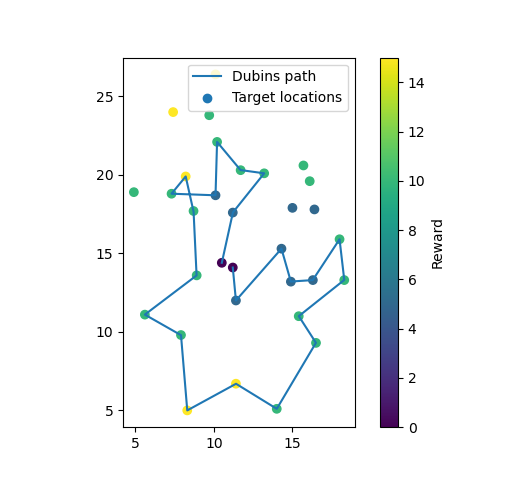
\includegraphics[width=7cm]{Set1_Dubinspath_rad0.png} }}%
	\qquad
	\subfloat[\centering Zulässige Lösung für $\rho = 1$, $T_{max} = 60$ mit Belohnung $R(P) = 150$]{{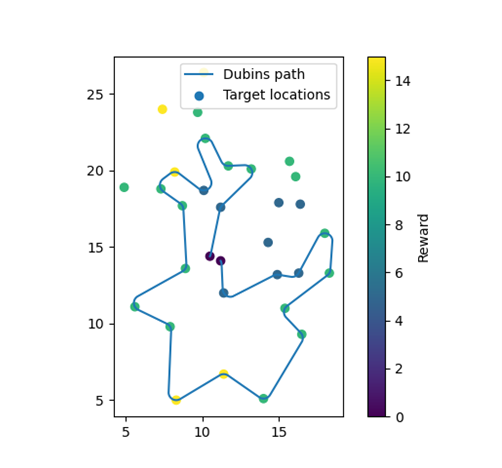
\includegraphics[width=7cm]{Set1_Dubinspath_rad1.png} }}%
	\caption{Probleminstanz Set 1 mit zwei zulässigen Lösungen}
	\label{fig:Set1_Dubinspath_rad01.png}
\end{figure}

\subsection{Testinstanz und verwendete Parameter}\label{subsection:testinstance}
Zur Evaluation des Verfahrens werden sowohl die Parameter des Dubins Orienteering Problems als auch die des Verfahrens selbst variiert.

Zunächst hat der minimale Kurvenradius $\rho$ einen großen Einfluss auf die resultierenden Lösungen des DOP. Dieser wird hier einmal als 0 angenommen, womit der Fall des regulären OP abgedeckt wird. Im anderen Fall wird $\rho = 1$ angenommen.
Im Fall $\rho = 0$ wird die Suche nach den optimalen Ausrichtungswinkeln $\Theta$ überflüssig, da die Dubinsdistanz aufgrund der unendlich großen Krümmung unabhängig von den Winkeln ist und zur euklidischen Distanz wird, welche nur noch von der Position der Ziele abhängt. Im Verfahren müssen folglich die Ausrichtungswinkel nicht mehr bestimmt werden und es reicht aus einen beliebigen Ausrichtungswinkel zu wählen ($m=1$), wodurch sich die Graphensuche erheblich beschleunigt.

Im Fall $\rho > 0$ bestimmt das Verhältnis zwischen Kurvenradius und den Abständen der Ziele, was für Lösungen und damit Belohnungen für welche Streckenbudgets zulässig sind. Für das Verfahren an sich hat der minimale Kurvenradius vor allem Einfluss auf die Anzahl der Ziele in einer zulässigen Lösung. Mit zunehmendem Kurvenradius werden die Dubinspfade zwischen den Zielen länger, was dazu führt, dass bei gleichem Streckenbudget weniger Ziele besucht werden können. Die Wahl $\rho = 1$ orientiert sich zur besseren Vergleichbarkeit an der zugrundeliegenden Arbeit \cite{R.Penicka.2017}.

Um das Verfahren dennoch für verschiedene Anzahlen an Zielen in den zulässigen Lösungen beurteilen zu können, wird das Streckenbudget $T_{max}$ variiert. Dabei werden die Werte 20, 40 und 60 eingesetzt, welche sich ebenfalls an der zugrundeliegenden Arbeit orientieren.

Ein weiterer Parameter, der Einfluss auf die Laufzeit des Verfahrens hat, ist die Anzahl $m$ der diskreten Werte, die die Ausrichtungswinkel $\Theta$ annehmen können. Je größer $m$ ist, desto besser ist die Approximation an den tatsächlich besten Dubinspfad durch eine gegebene Menge an Zielen, in dem beliebige Ausrichtungswinkel vorkommen können. Entsprechend können bessere Pfade geflogen werden, was dazu führt das sich die benötigte Distanz einer gegebenen Lösung verringert. Folglich können mehr Belohnungen eingesammelt werden.

Für größeres $m$ wächst allerdings auch der Suchgraph zur Bestimmung der optimalen Ausrichtungen, wodurch sich die Erzeugung dieses Graphen und die anschließende Suche in ihm erheblich verlängern. Da diese Graphensuche bei jedem Einfügen und Verschieben von Zielen erfolgt, verlängert sich auch die benötigte Zeit je Iteration erheblich.

In der zugrundeliegenden Arbeit wird gezeigt, dass in den Probleminstanzen bereits für $m = 4$ gut 80\% der Belohnungen erreicht werden, die für $m=20$ gefunden werden. Ab $m = 8$ sind keine nennenswerten Verbesserungen in den gefundenen Belohnungen mehr zu erwarten.
In dieser Arbeit werden daher die Werte $m = 4$ und $m = 8$ verwendet.

Penicka et al. \cite{R.Penicka.2017} finden ihre besten Lösungen nach 1000 bis 4000  Iterationen des Verfahrens. Da die Implementierung im Rahmen dieser Arbeit in \textit{Python} und insbesondere die Bestimmung der Ausrichtungswinkel nicht hinreichend performant ist, bleibt aus Laufzeitgründen die Anzahl der Iterationen auf 1000 beschränkt.

Die Variationen der Parameter sind in Tabelle~\ref{tab:Parametervariation} noch einmal zusammengefasst.

\begin{table}[h]
	\centering
	\begin{tabular}{ |c|c| }
		\hline
		Parameter & Werte \\
		\hline  
		Minimaler Kurvenradius $\rho$ & 0, 1 \\ 
		Streckenbudget $T_{max}$ & 20, 40, 60 \\
		Anzahl der Ausrichtungswinkel $m$ &  4, 8\\
		Anzahl der Iterationen der VNS & 1000\\
		\hline
	\end{tabular}
	\caption{Parameter des DOP und der VNS und zugehörige Werte}
	\label{tab:Parametervariation}
\end{table}

\subsection{Einflüsse auf die Laufzeit}\label{subsection:laufzeit}
Bevor die eigentliche Qualität der erhaltenen Lösungen beurteilt werden soll, werden zunächst die Laufzeit des Verfahrens und die wichtigsten Einflussfaktoren auf diese analysiert.

Die Integrated Development Environment \textit{PyCharm} welche zur Implemementierung verwendet wurde, besitzt eine \textit{Profiler}-Funktion, mit der einzelne sowie kumulierte Dauer aller Methodenaufrufe eines \textit{Python}-Skripts gemessen werden kann.

Die sich aus 1000 Iterationen der implementierten RVNS einschließlich vorhergehender Berechnung aller Dubinsdistanzen und Konstruktion einer initialen Lösung ergebenden Anteile der einzelnen Methoden an der Laufzeit finden sich in Tabelle~\ref{tab:Laufzeitanalyse}. Es sind alle Methoden aufgeführt, deren Eigenanteil an der Laufzeit mindestens 1.5\% beträgt.

\begin{table}
	\centering
	\begin{tabular}{ |c|c|c| }
		\hline
		Methode & Gesamtzeit & Eigene Zeit\\
		\hline
		bidirectional\textunderscore dijkstra & 44.2\% & 30.9\%\\
		add\textunderscore edge & 25.9\% & 21.4\%\\
		generate\textunderscore search\textunderscore graph & 53.4\% & 19.1\%\\
		get\textunderscore distance & 6.3\% & 6.3\%\\
		get (dict object) & 5.1\% & 5.1\% \\
		update (dict object) & 3.1\% & 3.1\% \\
		add\textunderscore node & 2.2\% & 1.9\%\\
		\hline
	\end{tabular}
	\caption{Methoden der Implementierung der VNS nach Eigenanteilen an der Laufzeit. Set 1, $\rho = 1$, $T_{max} = 40$, $m = 8$}
	\label{tab:Laufzeitanalyse}
\end{table}

Wie Tabelle~\ref{tab:Laufzeitanalyse} zu entnehmen ist, haben die Methoden, die für die Erzeugung des Suchgraphen zur Optimierung der Ausrichtungen (add\textunderscore edge, generate\textunderscore search\textunderscore graph, add\textunderscore node) einen gemeinsamen Eigenanteil von 42.4\% der Laufzeit. Die Suche nach dem kürzesten Pfad in diesem Graph per Dijkstra-Algorithmus (bidirectional\textunderscore dijkstra) hat zusätzlich noch einen Eigenanteil von 30.9\% an der Laufzeit. Insgesamt sorgt so die Optimierung der Ausrichtungen für 72.3\% des Rechenaufwandes.

Die Zugriffe auf die Dubinsdistanzen (get\textunderscore distance, get (dict object), update (dict object)) benötigen weitere 14.5\% des Rechenaufwandes.

\subsection{Ergebnisse}\label{subsection:results}
Die Ergebnisse für die Parametervariationen sind in Tabelle~\ref{tab:Results_Parametervariation} dargestellt.
Im Fall $\rho = 0$ ist $m = 1$ vermerkt, da aufgrund der unendlich großen maximalen Krümmung nur ein Ausrichtungswinkel betrachtet werden muss.

\begin{table}[h]
	\centering
	\begin{tabular}{ |c|c|c|c|c|c| }
		\hline
		$T_{max}$ & $\rho$ & $m$ &  Laufzeit (sec.) & $R(P)$ & $\mathcal{L}_d(P)$ \\
		\hline  
		20 & 0 & 1  & 76.19
		 & 35 & 14.8149\\
		20 & 1 & 4  & 493.91
		 & 25 & 14.4851 \\
		20 & 1 & 8  & 2355.01
		& 35 & 16.8174\\ 
		40 & 0 & 1  & 153.04
		 & 115 & 39.8056
		 \\
		40 & 1 & 4 & 919.47
		 & 95 & 37.2137
		 \\
		40 & 1 & 8  & 3497.79
		& 100 & 37.4516
		\\
		60 & 0 & 1  & 186.98
		 & 170 & 59.5229
		 \\
		60 & 1 & 4  & 1138.56
		& 150 & 57.7183
		\\
		60 & 1 & 8  & 4808.09
		& 170 & 59.7046
		\\
		\hline
	\end{tabular}
	\caption{Beste mit der VNS (1000 Iterationen) gefundene Lösungen des DOP auf Set 1 und zugehörige Laufzeiten}
	\label{tab:Results_Parametervariation}
\end{table}

Erwartungsgemäß nimmt mit dem Streckenbudget $T_{max}$ auch die Belohnung $R(P)$ sowie die Distanz der besten gefundenen Lösung zu. Dabei fällt auf, dass die Abstände zwischen der Distanz der gefundenen Lösung und dem Streckenbudget umso kleiner werden, je größer letzteres ist. Je größer das Streckenbudget $T_{max}$, desto kleiner sind relativ die Distanzen zwischen den Zielen. Somit nimmt auch der Einfluss der Distanz einzelner Ziele beim Hinzufügen zur Lösung ab, weshalb das Streckenbudget besser ausgeschöpft werden kann. Dies erklärt sich aus der Analogie des DOP bzw. OP zum Rucksackproblem \cite{Nickel.2014}. Je geringer die Gewichte der zu packenden Gegenstände relativ zur Kapazität des Rucksacks sind, umso besser lässt sich Letztere ausnutzen.

Mit steigender Anzahl $m$ der Ausrichtungswinkel nimmt die Belohnung der gefundenen Lösung bei gleichbleibender Distanz $\mathcal{L}_d(P)$ zu. Dabei stimmen für $T_{max} \in \{20,60\}$ die gefundenen Lösungen hinsichtlich ihrer Belohnungen für $m = 8$ sogar mit denjenigen für $\rho = 0$ überein. Lediglich im Fall $T_{max}$ fällt die Belohnung der Lösung des OP ($\rho = 0$) um 15\% höher aus als diejenige des DOP mit $m = 8$. Dafür ist in diesem Fall der Abstand der Belohnung für $m = 8$ zu derjenigen für $m = 4$ deutlich geringer als bei den anderen Streckenbudgets.

Für alle Streckenbudgets zeigt sich ein exponentieller Anstieg der für die 1000 Iterationen benötigten Laufzeit, wenn $m$ wächst. Dies hängt mit der schnell zunehmenden Größe des Suchgraphen für die Ausrichtungswinkel zusammen, welche dafür sorgt, dass der Aufbau des Graphen einerseits und die Pfadsuche darin andererseits länger dauern.

Die Laufzeit der VNS steigt ebenfalls mit dem Streckenbudget $T_{max}$ an. Dies rührt daher, dass die erzeugten Pfade für größere Budgets länger sind und entsprechend mehr Ausrichtungen optimiert werden.

Tatsächlich fallen die in dieser Arbeit erreichten Belohnungen für alle hier betrachteten Kombinationen von $T_{max}$, $\rho$ und $m$ deutlich geringer aus als die von Penicka et al. \cite{R.Penicka.2017} mit der VNS gefundenen, welche in Tabelle~\ref{tab:Results_Penicka} dargestellt sind.

\begin{table}[h]
	\centering
	\begin{tabular}{ |c|c|c|c| }
		\hline
		$T_{max}$ & $\rho$ & $m$ &  $R(P)$ \\
		\hline  
		20 & 0 & 1  & 65\\
		20 & 1.1 & 12  & 60\\ 
		40 & 0 & 1  & 155\\
		40 & 1.1 & 12 & 140\\
		60 & 0 & 1  & 220\\
		60 & 1.1 & 12  & 205\\
		\hline
	\end{tabular}
	\caption{Beste gefundene Lösungen von Penicka et al. \cite{R.Penicka.2017} für das DOP auf Set 1}
	\label{tab:Results_Penicka}
\end{table}


Einerseits verwenden die Autoren eine höhere Anzahl an Ausrichtungen von $m = 16$. Dadurch ist jedoch noch keine solch signifikante Steigerung der Belohnung zu erwarten.
Andererseits verwenden sie eine maximale Anzahl an Iterationen von 10000. Zusätzliche bricht das Verfahren ab, wenn seit 3000 Iterationen keine Verbesserung erzielt wurde. Obwohl Penicka et al. hierzu keine expliziten Angaben machen, deutet die hohe Schranke darauf hin, dass bei der VNS regelmäßig tausende von Iterationen vergehen, ohne dass eine verbesserte Lösung gefunden wird.

Mithilfe der dieser Arbeit zugrundeliegenden Implementierung kann diese Hypothese überprüft werden, indem die initial konstruierten Lösungen mit den besten über das ganze Verfahren hinweg gefundenen verglichen werden. Die initial konstruierten Lösungen sind in Tabelle~\ref{tab:Results_Parametervariation_Initial} dargestellt.

\begin{table}[h]
	\centering
	\begin{tabular}{ |c|c|c|c|c|c| }
		\hline
		$T_{max}$ & $\rho$ & $m$ &  Laufzeit (sec.) & $R(P)$ & $\mathcal{L}_d(P)$ \\
		\hline  
		20 & 0 & 1  & 0.11
		& 35 & 14.8149\\
		20 & 1 & 4  & 1.65
		& 25 & 14.4851 \\
		20 & 1 & 8  & 6.37
		& 35 & 16.8174\\ 
		40 & 0 & 1  & 0.33
		& 115 & 39.8056
		\\
		40 & 1 & 4 & 2.46
		& 95 & 37.2137
		\\
		40 & 1 & 8  & 10.07
		& 100 & 37.4516
		\\
		60 & 0 & 1  & 0.533
		& 170 & 59.5229
		\\
		60 & 1 & 4  & 4.29
		& 150 & 57.7183
		\\
		60 & 1 & 8  & 20.64
		& 170 & 59.7046
		\\
		\hline
	\end{tabular}
	\caption{Initial konstruierte Lösungen des DOP auf Set 1}
	\label{tab:Results_Parametervariation_Initial}
\end{table}

Es zeigt sich, dass in allen betrachteten Fällen nicht nur die Belohnungen sondern auch die Distanzen der besten im Laufe der VNS gefundenen Lösungen mit den initial konstruierten Lösungen übereinstimmen. Aus der angegebenen Genauigkeit der Distanzen folgt, dass es sich um die gleichen Lösungen handeln muss. Dies bedeutet, dass für keine der 9 Parameterkombinationen innerhalb von 1000 Iterationen eine verbesserte und zulässige Lösung gefunden werden konnte.
Die entsprechende if-Bedingung in Algorithmus~\ref{algo:VNS_DOP} ist nie erfüllt.

\subsection{Verbesserungsmöglichkeiten des Verfahrens}\label{subsection:possibleImprovement}
\subsubsection{Berücksichtigung der Zulässigkeit und Zeitpunkte der Ausrichtungsoptimierung}\label{subsubsect:headingoptimization}
Durch eine genauere Analyse des Programmablaufs lässt sich nachvollziehen, dass in der Mehrzahl der Fälle die gefundene Lösung zwar eine höhere Belohnung besitzt, sie aber aufgrund der zu großen Länge der Dubinspfade unzulässig ist.

Tatsächlich wird die Zulässigkeit der untersuchten Lösungen im Verfahren während \textit{shaking} und \textit{local search} nicht überprüft. Somit wird ausgehend von einer durch \textit{shaking} erzeugten, möglicherweise bereits unzulässigen, Lösung ausgehend lokal gesucht, wobei sich die Unzulässigkeit in jedem Schritt verändern kann. Weil die initial gefundenen Lösungen das Budget bereits relativ stark ausreizen, ist die Wahrscheinlichkeit einer unzulässigen Lösung durch das Verschieben einzelner Ziele recht hoch.

Eine Überprüfung der Zulässigkeit würde jedoch keine zusätzliche Laufzeit kosten, da bereits "`in jeder der Nachbarschaftsstrukturen die Operationen auch durch alle Ausrichtungswinkel suchen, [...] um die Pfadlänge für eine gegebene Sequenz an Zielen zu minimieren"'\cite{R.Penicka.2017}. Um mittels der optimalen Ausrichtungen die Zulässigkeit zu überprüfen muss anschließend nur noch die am Anfang des Verfahrens berechnete Länge des Dubinspfads nachgeschlagen werden, was wie in Abschnitt~\ref{subsection:implementation} beschrieben, keinen nennenswerten Aufwand bedeutet.
In jedem Fall ist die Ausrichtungsoptimierung in jedem Zwischenschritt unnötig, sofern nicht gleichzeitig die Zulässigkeit der Lösung überprüft wird.

Folglich bieten sich zwei Verbesserungsmöglichkeiten an.
Erstens kann die mit Laufzeit erworbene Information über die Zulässigkeit genutzt werden, um die lokale Suche zu steuern.
Zweitens kann auf die Ausrichtungsoptimierung verzichtet werden und nur eine belohnungsgesteuerte lokale Suche durchgeführt werden. Dadurch ließe sich die Anzahl der möglichen Iterationen stark erhöhen, da die Optimierung über die Ausrichtungen aufgrund des Aufbaus des Suchgraphen und der Pfadsuche in ihm den Großteil des Rechenaufwandes ausmacht. Die Ausrichtungsoptimierung wird dann lediglich zur Bestimmung der Zulässigkeit \textit{nach Abschluss} der lokalen Suche durchgeführt.

\subsubsection{Bestimmung der erreichbaren Ziele}\label{subsubsec:reachableLocations}
Eine weitere Verbesserungsmöglichkeit ist die Relaxierung der Bedingung~(\ref{eq:I_r}) an die erreichbaren Ziele $I_r$, die bereits in Abschnitt~\ref{subsection:construction} erwähnt wurde. Hier werden nicht nur diejenigen Ziele berücksichtigt, welche für alle Ausrichtungskombinationen erreichbar sind, sondern auch all jene, die für eine Ausrichtungskombination erreichbar sind. So soll vermieden werden, möglicherweise hilfreiche Ziele unnötigerweise bei der Konstruktion der initialen Lösung zu übergehen. Die basierend auf der relaxierten Bedingung konstruierten Lösungen finden sich in Tabelle~\ref{tab:Results_Parametervariation_Initial_notAllAngles}.

\begin{table}[h]
	\centering
	\begin{tabular}{ |c|c|c|c|c|c| }
		\hline
		$T_{max}$ & $\rho$ & $m$ &  Laufzeit (sec.) & $R(P)$ & $\mathcal{L}_d(P)$ \\
		\hline  
		20 & 0 & 1  & 0.11
		& 35 & 14.8241\\
		20 & 1 & 4  & 1.86
		& 35 & 16.5060 \\
		20 & 1 & 8  & 6.82
		& 35 & 15.4542\\ 
		40 & 0 & 1  & 0.34
		& 115 & 39.8339
		\\
		40 & 1 & 4 & 2.50
		& 95 & 37.2137
		\\
		40 & 1 & 8  & 10.69
		& 100 & 37.4516
		\\
		60 & 0 & 1  & 0.58
		& 170 & 59.5512
		\\
		60 & 1 & 4  & 4.45
		& 150 & 57.7183
		\\
		60 & 1 & 8  & 20.90
		& 170 & 59.7046
		\\
		\hline
	\end{tabular}
	\caption{Initial konstruierte Lösungen des DOP auf Set 1 mit relaxierter Bedingung an $I_r$}
	\label{tab:Results_Parametervariation_Initial_notAllAngles}
\end{table}

Gegenüber der nicht-relaxierten Bedingung an $I_R$, dargestellt in Tabelle~\ref{tab:Results_Parametervariation_Initial},
erhöht sich die Belohnung der initialen Lösung im Fall $T_{max} = 20$, $\rho = 1$, $m = 4$ von 25 auf 35. Alle anderen erzielten Belohnungen bleiben gleich. Im Fall $T_{max} = 20$, $\rho = 1$, $m = 8$ verringert sich die Distanz der initialen Lösung bei gleicher Belohnung um 1.3632 LE, während sich die Distanz im Fall $T_{max} = 20$, $\rho = 0$, $m = 1$ um 0.0092 LE leicht erhöht. Alle anderen Distanzen sind unverändert. Daneben ist ein leichter Anstieg der Laufzeiten zu beobachten, der mit der größeren Anzahl an Zielen in $I_r$, die bei der Konstruktion der initialen Lösung zu berücksichtigen sind, zu erklären ist.

Gerade für kleine Streckenbudgets wie $T_{max} = 20$ scheint sich die Relaxierung und damit einhergehende Vergrößerung von $I_r$ zu empfehlen, da hier die Forderung, dass ein Ziel für alle Ausrichtungskombinationen erreichbar sein muss, zu restriktiv ist. Die dafür notwendige Erhöhung der Laufzeit ist minimal.

Eine solche Ausweitung von $I_r$ hat jedoch auch während der Verbesserungsschritte Einfluss auf die Laufzeit des Verfahrens. Die Länge der Permutation $\Sigma$ entspricht im laufenden Verfahren gerade $|I_r|$, sodass die resultierenden Pfade im Erwartungswert länger werden. Dies führt einerseits dazu, dass der für die Ausrichtungsoptimierung verwendete Graph aufwendiger zu erzeugen und zu durchsuchen ist, da die Anzahl seiner Stufen im Erwartungswert mit der Permutationslänge zunimmt. Andererseits steigt mit der durchschnittlichen Pfadlänge auch die Wahrscheinlichkeit unzulässige Lösungen zu erzeugen. Zusätzlich erhöht sich aufgrund der längeren Permutation die Anzahl der Lösungen in jeder Nachbarschaft $N_l(P)$. Damit steigt bei einer systematischen lokalen Suche der Rechenaufwand in jeder Iteration. Bei der randomisierten VNS wird entweder die Anzahl der zufälligen Verbesserungsversuche mit $|I_r|^2$ angehoben, wobei sie quadratisch zunimmt. Oder sie bleibt gleich, was dazu führt, dass zwar der Rechenaufwand gleich bleibt, die größere Nachbarschaft aber spärlicher durchsucht wird.

Zusammenfassend muss, bei der Entscheidung, nach welcher Bedingung $I_r$ erzeugt wird, die Erhöhung in der zu erwartenden Belohnung der initialen Lösung gegen die zu erwartende Erhöhung der Laufzeit jeder einzelnen Iteration abgewogen werden.

\subsubsection{Konstruktion der initialen Lösung}\label{subsubsec:constructionImprove}
Angesichts der sehr geringen Wahrscheinlichkeit einer Verbesserung jeder Iteration kommt der initial konstruierten Lösung eine besondere Bedeutung zu. Wie in Abschnitt~\ref{subsection:construction} beschrieben, besteht in der zugrundeliegenden Arbeit der Ansatz zur Konstruktion der initialen Lösung darin, basierend auf einem initial leeren Lösung iterativ diejenigen Ziele hinzuzufügen, deren Verhältnis zwischen Belohnung und zusätzlicher Distanz maximal ist. 

Diese Vorgehensweise ist äquivalent zur ersten Phase der vierphasigen Heuristik von Ramesh et al. \cite{Ramesh.1991}.
Anstatt nach dieser bereits die eigentliche VNS zu starten, können noch weitere Phasen dieser Heuristik zur Verbesserung der Lösung eingesetzt werden. Dazu zählen die zweite Phase, in der 2- und 3-OPT Operationen ausgeführt werden sowie die dritte Phase, in der basierend auf dem Verhältnis aus Belohnung und zusätzlicher Distanz Ziele aus der Lösung entfernt werden.

Zuletzt können in der vierten Phase bisher vernachlässigte Ziele hinzugefügt werden. Dieses wird im Rahmen der VNS durch die zufälligen Einfügeoperationen bereits verwirklicht, jedoch erfolgt dies nicht gezielt für Ziele außerhalb der Lösung sondern diese werden aus der gesamten Permutation ausgewählt. Weiterhin wird in der VNS mit einer Lösung begonnen, die das Budget bereits annähernd ausschöpft. Die Löschung einiger Ziele aus der Lösung kann daher sinnvoll sein, um nach dem hinzufügen vernachlässigter Ziele eher eine zulässige Lösung zu erhalten.

\subsubsection{Verwendung geometrischer Informationen zur Verbesserung einer Lösung}\label{subsubsec:useGeometry}
Die Operationen der VNS verwenden keine Informationen über die Lage der Ziele zueinander, da nur deren Reihenfolge in der Permutation verändert wird. Diese geometrischen Informationen können allerdings hilfreich sein, um zu entscheiden, welche Ziele einer Lösung hinzugefügt werden sollen. So könnte beispielsweise eine Nachbarschaftsstruktur der VNS hinzugefügt werden, in der jeweils der nächste Nachbar aller Ziele in der Lösung vorhanden ist, was dazu führt, dass nur dem Pfad bereits nahe Ziele hinzugefügt werden. Diese heben die Distanz der Lösung in der Tendenz weniger stark an als Ziele, die weit vom Pfad entfernt liegen. Somit könnten mehr zulässige Lösungen erzeugt werden.

Auch für die Ausrichtungsoptimierung könnte die Lage der Ziele herangezogen werden. Statt einer vollständigen Suche nach den optimalen Ausrichtungen kann beim Hinzufügen eines neuen Ziels als Heuristik der Mittelwert der Ausrichtungen von Vorgänger- und Nachfolgerziel verwendet werden. Vollständige Optimierungen könnten dann in regelmäßigen aber größeren Abständen zur Zulässigkeitskontrolle eingesetzt werden, wodurch die Laufzeit der einzelnen Iterationen gesenkt wird.

\subsubsection{Modifikation des Suchgraphen}\label{subsubsec:modifySearchGraph}
Nach den Beobachtungen aus in Abschnitt~\ref{subsection:laufzeit} sorgt allein die Erzeugung des Suchgraphen zur Ausrichtungsoptimierung für 42.4\% der gesamten Laufzeit des Verfahrens und benötigt sogar noch mehr Zeit als die anschließende Pfadsuche. Daher liegt es nahe, diesen Zeitaufwand zu reduzieren. In der dieser Arbeit zugrundeliegenden Implementierung wird für jede neu erzeugte Lösung erneut der Suchgraph basierend auf den Dubinsdistanzen und der entsprechenden Permutation $\Sigma$ aufgebaut. Dies erfolgt erst nachdem die Verschiebe- und Einfügeoperationen ausgeführt wurden.

Alternativ können die Implementierungen der Verschiebe- und Einfügeoperationen so verändert werden, dass diese nicht nur die Permutation der Ziele verändern, sondern auch den Suchgraphen der bisherigen Lösung verändern. So muss kein neues Objekt erzeugt werden und nur ein kleiner Anteil der Kanten des Graphen entfernt und neu hinzugefügt werden, nämlich an den Stellen, wo neue Ziele und Teilpfade eingefügt und entfernt wurden.

Damit lässt sich der Rechenaufwand zur Erstellung des neuen Suchgraphen erheblich reduzieren.

\newpage

\section{Zusammenfassung}\label{section:conclusion}
In der vorliegenden Arbeit wurde das Dubins Orienteering Problem als Synthese des klassischen Orienteering Problems mit dem kinematischen Modell des Dubinsfahrzeugs vorgestellt sowie ein kurzer Überblick über die wichtigste Literatur gegeben. Anschließend wurde ein zur Lösung des DOP angepasstes Verfahren, basierend auf der variablen Nachbarschaftssuche (VNS), präsentiert. Mittels einer eigenen Implementierung in \textit{Python} wurde dessen Verhalten auf einer bekannten Testinstanz überprüft.

Anhand der numerischen Ergebnisse und theoretischen Überlegungen wurden die Anwendbarkeit des Verfahrens diskutiert und verschiedene Verbesserungsmöglichkeiten aufgezeigt.\\

Wie diese Arbeit zeigt, handelt sich bei der VNS um ein Verfahren, welches einer sehr hohen Anzahl an Iterationen bedarf, um die sehr seltenen zulässigen Verbesserungsschritte zu realisieren.

Dies impliziert erstens, dass die initial konstruierte Lösung so gut wie möglich sein sollte, wofür einerseits mehr erreichbare Ziele herangezogen werden können und andererseits weitere Heuristiken wie die vierphasige Heuristik der VNS vorgeschaltet werden können.

Zweitens sollte die Laufzeit der einzelnen Iterationen der VNS gesenkt werden. Einerseits durch Reduzierung der Häufigkeit der in weiten Teilen des Verfahrens unnötigen Ausrichtungsoptimierung. Andererseits durch Beschleunigung dieser mittels einer Modifikation des Suchgraphens sowie durch eine generell effizientere Implementierung mit effizienten Bibliotheken und Programmiersprachen.

Zuletzt kann durch weitere angepasste Nachbarschaftsstrukturen und Heuristiken zur Ausrichtungsoptimierung vorliegende geometrische Information eingesetzt werden um die Wahrscheinlichkeit zulässiger Lösungen zu erhöhen und die Iterationen zu beschleunigen.\\

Der Schlüssel zum gewinnbringenden Einsatz dieses  Verfahrens liegt somit einerseits in effizienten Iterationen zum schnellen Erreichen einer hohen Iterationszahl und andererseits in einer möglichst hohen Wahrscheinlichkeit verbesserte und zulässige Lösungen zu generieren.

\newpage
%-------------------------------------------------------------------------------------------------------------------

%-----------------------------------------------------------------------------------------------------------------------------
%Abbildungsverzeichnis
\listoffigures
\addcontentsline{toc}{section}{Abbildungsverzeichnis}
\newpage
%Tabellenverzeichnis
\listoftables
\addcontentsline{toc}{section}{Tabellenverzeichnis}
\newpage
%Literaturverzeichnis
\renewcommand\refname{Literaturverzeichnis}
\bibliography{Literatur.bib} 
\bibliographystyle{plainurl}
\addcontentsline{toc}{section}{Literaturverzeichnis}

\end{document}